%%%%%%%%%%%%%%%%%%%%%%%%%%%%%%%%%%%%%%%%%%%%%%%%%%%%%%%%%%%%%%%%%%%%
% Diskussion und Ausblick
%%%%%%%%%%%%%%%%%%%%%%%%%%%%%%%%%%%%%%%%%%%%%%%%%%%%%%%%%%%%%%%%%%%%

\chapter{Applications}

\section{Command Line Interface}\nomenclature{CLI}{Command Line Interface}\index{CLI}\index{Command-Line Interface}\label{cli}
Almost every script needs some informations. An information which every scripts need is key and token of the user which account should be used for the access to Trello. The scripts have to know which cards, lists and boards they have to look at. So these information has to be passed to the scripts, too. At first we set this information at the top of the script. But it emerged that it's very unpractical to hard code this in each script. So it would be impossible to use the same Ruby file with several Trello accounts. For every Trello account the user has to generate a dedicated file. The solution for this problem is a command-line interface (CLI). With a CLI the user can pass information to the script in a predefined format, so the script knows exactly what to do. For every other call the user can specify different information for one and the same script.

The Ruby class OptionParser\cite{ruby:optionparser} provides easy customisable command-line option analysis. The developer is able to specify its own options for each script. For this purpose a dedicated class is used. 
In order to let the actual script \emph{know} about the CLI arguments the developer has to require the respective CLI class with the command-line option definitions.

\begin{lstlisting}[aboveskip=1\baselineskip, style=bash, caption=Example usage of a script with CLI., label=listing004]
ruby html.rb -c 4ffd78a2c063afeb066408b8
\end{lstlisting}

An example usage of a script with CLI would look like Listing \ref{listing004}. The \texttt{-c} is an comman-line option. If there is a string behind the option, like in this case, the string is a so called \emph{argument}. But there are command-line options which stand for its own. Those are called \emph{flags}. Flags are only for polar decisions.

\begin{lstlisting}[aboveskip=1\baselineskip, caption=Definition of a command-line option, label=listing002]
# Trello list(s)
opts.on("-l", "--lists x,y,z", Array, "Ids of one or more Trello lists.") do |lists| (*@\label{line001}@*)
	options.lists = lists
end
\end{lstlisting}

Listing \ref{listing002} shows the definition of the option \texttt{-l} for passing one or more IDs of lists to a script. In Line \ref{line001} the word \lstinline{Array} casts the list argument to an Array object.

OptionParse provides an automated help option. If the user types 
\begin{center}
\texttt{ruby script.rb -h} 
\end{center}
he gets the explanation the developer wrote in the CLI class for this script with all possible options. This list ist automatically generated by the definitions of the command-line options like in Listing \ref{listing002}. It works with \texttt{-help} and \texttt{--help} instead of \texttt{-h}, too.

\begin{lstlisting}[aboveskip=1\baselineskip, style=bash, caption=Output of the \texttt{-h} option., label=listing003]
Usage: ical.rb [options]
Select the input cards with -c, -l, -b or -a

Specific options:
 -a, --[no-]all         Set this if all due dates of all cards of all boards this user can see shall be used.
 -l, --lists x,y,z      Ids of one or more Trello lists.
 -b, --boards x,y,z     Ids of one or more Trello boards.
 -c, --cards x,y,z      Ids of one or more Trello cards.
 -k MANDATORY, --key    Your Trello key.
 -t MANDATORY, --token  The Trello token.
\end{lstlisting}

Listing \ref{listing003} shows the Output of \texttt{ruby ical.rb -h}. 
These are the basic CLI commands used by every script. For some scripts there are additional commands. They are explained in their respective sections.

\section{Export to HTML}\nomenclature{HTML}{Hyper Text Markup Language}

Used libraries:
\begin{itemize}
	\item \texttt{erb}
	\item \texttt{json}
	\item \texttt{rest\_client}
	\item \texttt{pp}
	\item \texttt{kramdown}
\end{itemize}

The \texttt{html.rb} script exports the data of one ore more cards to an HTML file. The resulting HTML file lists the cards one below another. The order is determined by the order in the command-line argument. If the command-line looks like listing \ref{listing005} the script will process the list with the id \texttt{4ffd78ff7f0c71780cc5aa1c} at first. That means in the HTML file are all cards in this list and below these the single card with the id \texttt{4ffd78a2c063afeb066408b8}. In addition to the command-line options described in section \ref{cli} the option \texttt{--title} is used. Here the user has to specify a title for the web page. The title will be displayed at the top of the page in \lstinline{<h1>} HTML tags.

\begin{lstlisting}[aboveskip=1\baselineskip, style=bash, caption=Example for a \texttt{html.rb} call., label=listing005]
ruby html.rb -l 4ffd78ff7f0c71780cc5aa1c                 -c 4ffd78a2c063afeb066408b8 --title 'Madness'
\end{lstlisting} 

Each card is displayed with all their information. This includes title, description, members, due date, labels, votes, checklists, comments and attachments.

Trello itself distinguishes between photos and other attachments. Normal attachments are linked under the description. Photos are embedded in the HTML code as thumbnails. Trello detects JPEG, GIF and PNG files as pictures and displays them as thumbnails. In addition to these formats the resulting HTML file displays TIFF, PSD, BMP and JPEG2000 as thumbnails, too. All modern Browsers support these formats.

This script generates static HTML. Of course the goal could also reached with a dynamic solution with PHP or Ruby on Rails. But the upside is, that the user of the respective website hasn't to wait for the webserver. Dynamic websites are mostly fast in the meanwhile, but with static HTML files the developer is on the safe side. Especially if the data to be displayed doesn't change every minutes this approach pays off. The server hasn't to generate the whole data with every visit. It has just to send the static HTML files.

\subsection{Markdown}\index{Markdown}
Markdown is a small lightweight plain text formatting snytax, designed by John Gruber. It's designed for the use with blogs and CMS\nomenclature{CMS}{Content Management System}. In these use cases HTML is often too much. Markdown represents most of the features of HTML that are needed for writing. The designer of Markdown, had the goal that a text, written in Markdown, is still easy to read. John Gruber provides a software tool, written in the Perl programming language, that converts the Markdown formatted text to valid HTML. \cite{markdown}

\begin{lstlisting}[aboveskip=1\baselineskip, style=bash, caption=Example for a text written in Markdown., label=listing006]
### iCloud:(*@ \label{line002} @*)

1.   Shared Photo Streams Now you can *share* just the **photos** you want, with just the people you choose. (*@ \label{line003} @*)
2.   Reminder

------------------------------- (*@ \label{line004} @*)

Here is an example of AppleScript:

    tell application "Foo" (*@ \label{line005} @*)
        beep
    end tell

![Apple logo](http://upload.wikimedia.org/wikipedia/commons/f/fa/Apple_logo_black.svg "Apple logo") (*@ \label{line006} @*)
\end{lstlisting}


\begin{lstlisting}[aboveskip=1\baselineskip, style=html, caption=Listing \ref{listing006} converted to HTML., label=listing007]
<h3>iCloud:</h3>

<ol>
	<li>Shared Photo Streams Now you can <em>share</em> just the <strong>photos</strong> you want, with just the people you choose.</li>
	<li>Reminder</li>
</ol>

<hr>

<p>Here is an example of AppleScript:</p>

<pre>
	<code>tell application "Foo"
	beep
	end tell</code>
</pre>

<p><img alt="Apple logo" title="Apple logo" src="http://upload.wikimedia.org/wikipedia/commons/f/fa/Apple_logo_black.svg"></p>
\end{lstlisting} 

Listing \ref{listing006} shows a small example of Markdown. The \lstinline{###} in line \ref{line002} is a header equal to \lstinline{<h3>} in HTML. The first list item of the ordered list in line \ref{line003} contains italic and bold words. In line \ref{line004} is a horizontal line. After a normal line of text a code block starts in line \ref{line005}. At the end in line \ref{line006} there is a picture with title and alt texts. After the conversion it looks like listing \ref{listing007} in HTML. The appearance, of course, depends on the used CSS on the respective websites. The appearance in Trello is like in figure \ref{fig:markdown-result}.

\begin{figure}[htb]
\centering
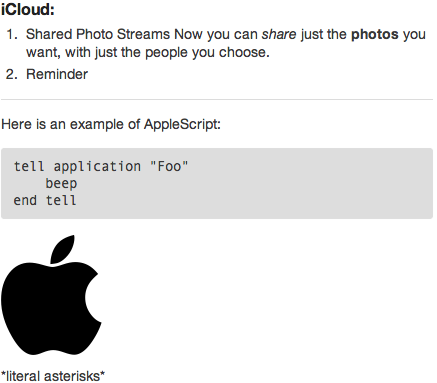
\includegraphics[scale=0.6]{figures/markdown-result}
\caption{The browser view of the HTML converted from the Markdown in listing \ref{listing006}}
\label{fig:markdown-result}
\end{figure}

Meanwhile Markdown became quite popular. Many blogging platforms support it, at least there are Markdown plug-ins for most platforms. Trello supports it in the description of cards. In the unlikely case that markdown reaches its limits inline HTML can be used. The only restriction ist, that HTML block-level-elements have to be separated to the previous and following Markdwon blocks.

For converting Markdown to HTML the gem kramdown is used. Figure \ref{fig:kramdown} decribes the convert options of kramdown. It converts to LaTeX and a special kramdown format, too. The kramdown format is an extended Markdown syntax. As input formats it accepts HTML and kramdown besides standard Markdown. \cite{kramdown} These additional features of kramdown might be useful for future approaches. To generate lists bibliographies for scripts, papers or books.

\begin{figure}[htb]
\centering
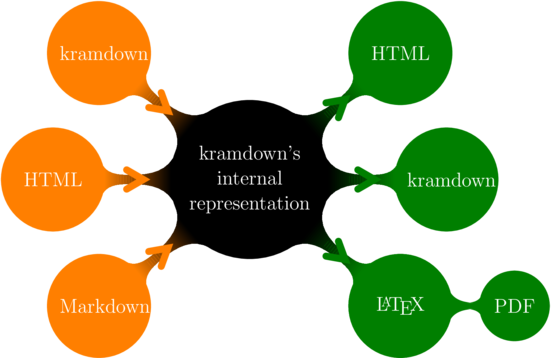
\includegraphics[width=\textwidth]{figures/kramdown}
\caption{Overview about kramdowns converting options. \cite{kramdown}}
\label{fig:kramdown}
\end{figure}

\subsection{Twitter Bootstrap Framework}\index{Twitter}\index{Bootstrap}
In 2011 Twitter released Bootstrap\footnote{Blog post by Mark Otto: \url{https://dev.twitter.com/blog/bootstrap-twitter}}. Bootstrap is a collection of methods and script for creating front-ends of websites. It contains templates for site structuring, tables, text, buttons, menus, forms, lists and some other often used elements of websites. Additionaly some functions are supported with JavaScript\index{JavaScript}. Bootstrap is written in HTML\index{HTML}, JavaScript, CSS\index{CSS} and LESS\index{LESS}. LESS is a dynamic stylesheet language and extends CSS. That allows the use of varables, functions, nested selectors and operators.\cite{less} Bootstrap is completely free of charge and open source. \cite{bootstrap}

Bootstrap\index{Bootstrap} evolved at Twitter\index{Twitter} while working on several projects with different libraries. The projects became inconsistent and a high administrative effort was needed. Some developers at Twitter lead by Mark Otto worked on something to document and share common design within the company. Twitter determined that this toolkit could be more than an intern helper tool. So they rouned it up with all common function which are needed for modern web development and released it on GitHub. \cite{markotto}

\subsection{HTML5}\index{HTML!5}
Twitter Bootstrap supports HTML5. HTML is the markup language for displaying content in a web browser. HTML5 is the latest revision of the HTML standard. It's an open format developed by the World Wide Web Consortium (W3C)\index{World Wide Web Consortium}\index{W3C}. HTML5 is a working draft since 2008. In 2011 the HTML Working Group at W3C advanced HTML5 to Last Call. So right now HTML communities all over the world are asked to confirm the starndard.  It is estimated that HTML5 will reach W3C Recommendation by 2014.\cite{html:lastcall} Although it is not yet finished, it is already widely used.

Before HTML5  there were two popular standards: HTML4\index{HTML!4} and XHTML1\index{XHTML}\nomenclature{XHTML}{Extensible Hyper Text Markup Language}. XHTML1 defines a XML\index{XML} serialisation for HTML4. With HTML5 there is only one language called HTML. This language can be written in HTML syntax and XML syntax. 
\cite{html:5differences} The W3C realised early the importance og smartphone in the future. They guided the development of HTML5 with the consideration of being able to run on low-powered devices. The market share of HTML5 enabled devices is still rising. \cite{smartphonesales} Smartphone sales even beat PC sales in 2012. Thus, it is increasingly important that web apps work well on small devices. To ensure this HTML5 is used. The foundation created here can therefore be used as a basis for the future.

HTML5 introduces several new elements. Some of the are usen in \texttt{html.rb}. At first there is the \lstinline{<header>} element. A header is an area at the top of a web page. It is used for navigational aids, logos or a search bar. \cite{html5:header} At the bootom is the \lstinline{<footer>} element. The \lstinline{<footer>} element can be used as a side wide footer and as a footer of sections. \cite{html5:footer} Here it is just used as side wide footer as preparation for data like licencing information, imprint and informations about the author. The cards are enclosed in \lstinline{<article>} elements. Every single card is represented as an \lstinline{<article>} element. That makes sense because typicalle a card is an article, especially if the user wants the card to be displayed on a web page. The W3C writes as requirements for a \lstinline{<article>} element that is has to be self-contained. \cite{html5:article} A card is a collection of information which is ordered by the several types of data. 

This foundation of generating HTML out of Trello can be used in various ways. It's predestinated for website with recuring kinds of information. Every business card style web page can definitely be managed with this script. From very small websites through to whole blogs could build on it.

\subsection{Templating with ERB}\index{ERB}\index{Templating}\nomenclature{ERB}{embedded Ruby}
Every card is embedded in the same HTML structure. Templates specify this HTML without the actual data. Instead of the data there is just a wildcard and a few control structures. Templating systems are used to organise the source code in operationally-distinct layers. The design is completely handled in the template file. But the control structure is partially in the template file, too. For a true separation of presentation of the data models and the logic components template engines, however, are unsuitable and there are additional concepts such as Model View Controller required (MVC)\nomenclature{MVC}{Model View Controller}.

ERB is a templating system for Ruby. It's part of the Ruby standard library. ERB accepts every string as a template, no matter if it is stored in a file, a database or some other kind of storage. ERB mainly used for generating HTML files. It is also able to generate any other kind of structured text, like RSS\index{RSS}\nomenclature{RSS}{Really Simple Syndication} feeds and XML\index{XML}. \cite{erb:introduction} \cite{erb:docu}

While generating the HTML ERB copies the plain text portions of the template file directly to the resulting document.  The parts which ERB has to process are marked with certain tags listed in listing \ref{listing011}
\begin{lstlisting}[aboveskip=1\baselineskip, style=bash, caption=Recognised tags in ERB., label=listing011]
<% Ruby code -- inline with output %>
<%= Ruby expression -- replace with result %>
<%# comment -- ignored -- useful in testing %>
% a line of Ruby code -- treated as <% line %> 
%% replaced with % if first thing on a line and % processing is used
<%% or %%> -- replace with <% or %> respectively
\end{lstlisting}
Only the first two tags are used here. The optimum would be if only \lstinline{<%= Ruby expression -- replace with result %>} would be used. Because that would imply that there are no control structures in the template file, just wildcards for data.

An real example of an ERB template is listing \ref{listing012}.

\begin{lstlisting}[aboveskip=1\baselineskip, caption=Ruby method in ERB template., label=listing012]
<small><%= getDate(card['due'], format='de') %></small>
\end{lstlisting}

A Ruby method is used as wildcard here. When processing the template file the method will be executed with the given variables and the result will be copied in the HTML file. But there are control structures, too. The block around the line in listing \ref{listing012} i showed in listing \ref{listing013}

\begin{lstlisting}[aboveskip=1\baselineskip, caption=Ruby method in ERB template., label=listing013]
<% if card['due'] %>
	<small><%= getDate(card['due'], format='de') %></small>
<% end %>
\end{lstlisting}

The \lstinline{if} construct is embedded with the \lstinline{<% ... %>} tag for ERB. Thats because it's not a wildcars which is replaced with actual content. This tag is just for control structures.

The alternative to using a templating system is to write the HTML at the same time and in the same file when the data is processed. That would result in a very confusing file which produces equally confusing HTML code. If the developer makes sure that the HTML code is well-structured the source code in the script looks even messier. That's because character escape codes like \lstinline{\t} and \lstinline{\n} have to be inserted manually in the source code. Otherwise the templating system takes this task. An example of such a confusing mixing of HTML, character escape codes and Ruby is shown in \ref{listing014}.

\begin{lstlisting}[aboveskip=1\baselineskip, caption=Generating HTML without a templating engine., label=listing014]
htmlSite << "</strong></span></p>
	\t\t\t\t<div style=\"text-align: left; padding-left: 5px;\"><span style=\"font-size: xx-small;\">"
htmlSite << description		
htmlSite << "</span></div>
	\t\t\t\t<div style=\"text-align: left;\"><span style=\"font-weight: normal; font-size: small;\"> 
	\t\t\t\t\t\t<ul>"
if element.attachments != []
	attachments.each do |attachment|
		name = attachment.name
		url = attachment.url
		htmlSite << "\t\t\t\t\t\t\t\t<li><a href=\""
		htmlSite << url
		htmlSite << "\">"
		htmlSite << name
		htmlSite << "<a/></li>"
	end	
end	
\end{lstlisting}

To represent the list of cards with the title in Ruby there is the Ruby class \texttt{webpage}. It is defined in listing \ref{listing015}.

\begin{lstlisting}[aboveskip=1\baselineskip, caption=Generating HTML without a templating engine., label=listing015]
class Webpage
  def initialize( title )
    @title = title

    @cards = [ ]
  end

  def add_card( card )
    @cards << card
  end

  def get_binding
    binding
  end
end
\end{lstlisting}

There are three methods. The \lstinline{initialize( title )} method generates the actual instance of the class. The instances modeled after this method contain the given title and an empty array for the cards. The \lstinline{add_card( card )} method simply adds a new card to the \lstinline{@cards} array. The last method is \lstinline{get_binding}. It generates a \lstinline{Binding} object of the current local variables.

\begin{lstlisting}[aboveskip=1\baselineskip, caption=Generating HTML with ERB., label=listing016]
templateFile = File.open("templateHtml.html.erb", "rb")(*@ \label{line007} @*)
template = templateFile.read

rhtml = ERB.new(template)(*@ \label{line008} @*)

webpage = Webpage.new( @htmlTitle )(*@ \label{line009} @*)

cardsFull.each do |card|(*@ \label{line010} @*)
  webpage.add_card(card)
end

html = rhtml.result(webpage.get_binding)(*@ \label{line011} @*)

fileHtml = File.new("index.html", "w+")(*@ \label{line012} @*)
fileHtml.puts html
fileHtml.close()
\end{lstlisting}

In listing \ref{listing016} the template data is set up. At first in line \ref{line007} the template file is opened in the next line read and saved in the \lstinline{template} variable. So the template is saved as string in \lstinline{template}. In line \ref{line008} with \lstinline{rhtml} an instance of ERB is created. After that in line \ref{line009} the \lstinline{Webpage} class is used. One instance with the given title is generated. In line \ref{line010} each card is added to the instance of \lstinline{Webpage}. Finally in line \ref{line011} the \lstinline{Binding} object of \lstinline{webpage} is created. With the ERB method \lstinline{result} the data in the \lstinline{Binding} object and the template come together. This is the step where the wildcards in the template file get filled with the actual data of the \lstinline{Binding} object. The resulting HTML code is saved in the string variable \lstinline{html} and \lstinline{html} is saved to the file \texttt{index.html} in line \ref{line012}. 

\section{Sync Google Calendar}\index{Google!Calendar}
Used libraries:
\begin{itemize}
	\item \texttt{erb}
	\item \texttt{json}
	\item \texttt{rest\_client}
	\item \texttt{pp}
	\item \texttt{google/api\_client}
\end{itemize}

Google Calendar is a free web service by Google for time-management. The service can be enabled in several calendar applications such as Apple Calendar (it was called iCal prior to Mac OS X 10.8) and Microsoft Outlook. Even all important mobile operating systems support it. Google Calendar it one of the most popular calendar web services. One advantage over other offferings is the excellent integration with all the other Google services which of most are very popular, too.

Google provides an API to access Calendar. There is even an API wrapper for Ruby made by Google. But ether it is very buggy or the documentation is poorly written. Some parameters the documentation says are available to send an API call at aren't actually available. Google grants normal developers a courtesy limit of 10,000 requests per day. Developers who need more requests per day for their application have to negotiate with Google and to contract about a higher request rate.

\begin{lstlisting}[aboveskip=1\baselineskip, caption=Initialisation of the Google Calendar API connection., label=listing017]
client = Google::APIClient.new
client.authorization.client_id = ' '
client.authorization.client_secret = ' '
client.authorization.scope = 'https://www.googleapis.com/auth/calendar'
client.authorization.refresh_token = ' '
client.authorization.access_token = ' '

result = client.authorization.fetch_access_token!
client.authorization.access_token = result['access_token']

service = client.discovered_api('calendar', 'v3')
\end{lstlisting}

Authetication with Google is much more complicated than with Trello. Listing \ref{listing017} shows the initialisation of the Google Calendar API connection. At first the project has to be registered in the Google APIs Console. \cite{google:apisconsole} There the developer can get the \lstinline{client_id} and the \lstinline{client_secret}. The \lstinline{scope} depends on the Google APi the developer wants to use. Here it is \texttt{https://www.googleapis.com/auth/calendar} of course. \cite{google:apiscope} To get the \lstinline{access_token} this URL must be called: 
\begin{center}
\lstinline{https://accounts.google.com/o/oauth2/auth?scope=https%3A%2F%2Fwww.googleapis.com%2Fauth%2Fcalendar&redirect_uri=https%3A%2F%2Foauth2-login-demo.appspot.com%2Fcode&response_type=code&client_id=812741506391.apps.googleusercontent.com&access_type=offline}
\end{center}

If the request succeeds the response is as noted in listing \ref{listing018}.

\begin{lstlisting}[aboveskip=1\baselineskip, caption=Response of the token request., label=listing018]
{
  "access_token":"1/fFAGRNJru1FTz70BzhT3Zg",
  "expires_in":3920,
  "token_type":"Bearer",
  "refresh_token":"1/xEoDL4iW3cxlI7yDbSRFYNG01kVKM2C-259HOF2aQbI"
}
\end{lstlisting}

It's important to store the refresh token. If the application looses the refresh token, the API calls will no longer work. The user, or in this case the developer, has to obtain a refresh token manually again. \cite{google:calapi}

For the sync to Google Calendar only cards with a due dated are considered. At first the script instructs the API wrapper to get all cards. Sadly the Trello API provides no filter method to get only the cards with a due date. The next step is to check if the cards have due dates. If a card has a due date the script checks if this card is already added as an event in Google Calendar. To do so the Google library looks after this card on the basis of its id. If it's not already in Google Calendar the script has to add a new event to Google Calendar.

\begin{lstlisting}[aboveskip=1\baselineskip, caption=Adding a new event to Google Calendar., label=listing022]
event = { (*@ \label{line013} @*)
	'summary' => card['name'],
	'description' => card['desc'],
	'location' => card['id'],
	'start' => {
		'dateTime' => getDate(card['due'], format='iso8601'),
		'timeZone' => 'Europe/Berlin'
	},
	'end' => {
		'dateTime' => getDate(card['due'], format='iso8601'),
		'timeZone' => 'Europe/Berlin'
	}
} (*@ \label{line014} @*)

insertevent = client.execute(:api_method => service.events.insert, (*@ \label{line015} @*)
								:parameters => {'calendarId' => 'primary'}, (*@ \label{line016} @*)
								:body => JSON.generate(event),
								:headers => {'Content-Type' => 'application/json'})
\end{lstlisting}

At first a new \lstinline{event} object has to be created. That happens in listing \ref{listing022} in lines \ref{line013} to \ref{line014}. A hash is used for that. The received information about a card from Trello is stored in a hash. So to get the information \lstinline{card['KEYWORD']} is used, where \lstinline{KEYWORD} stands for the respective name of the cards field that is needed. In the location field of an event the script stores the card id. That's not exactly the correct kind of data to put in a location field. But to determine if a card is already represented as an event in Google Calender the script has to use any unique identifier. Since there is no location for Trello cards anyway, the location field can be used. Sadly Google doesn't provide any \emph{hidden} fields which developers can use for such purposes.

From line \ref{line015} is where the actual request happens. The \lstinline{service.events.insert} tells the Google API which method the developer wants to adress. \cite{google:calapi} In this case it's the method to insert a new event to an existing calendar. In line \ref{line016} the developer has to specify the id of the calendar in which the new event should apper. Clearly \texttt{primary} is not an id. \texttt{primary} stands for the primary calendar. In Google Calendar the user can create several calendars for different purposes. One for work, one for private stuff and so forth. So \texttt{primary} is a valid value, too. In the following line the body is being sent. To do that the \lstinline{event} object created before has to be converted to a JSON string. This is achieved by the \lstinline{generate} method of the JSON class. \cite{json:docu} In the last line of listing \ref{listing022} the Google API is told that the body of this request is formatted as JSON.

If the event is already inserted in the calendar the script checks if the card's summary, description or due date have changed since the last sync to Google Calendar. But before it checks back if this event really is the representation of the actual card. The Google API provides no method to search for events with a special location. So it isn't possible to search in the location of an event. The script looks in all fields of an event for the id of the corresponding Trello card. To ensure that the currently handled card is the same the currently handled event is the representation for, the script compares the location field of the event and the card id. If the comparison matches it runs almost the same code as in listing \ref{listing022}. But this time the Google Calendar API method which is used for updating the event is called \lstinline{service.events.update}. 

The third possible scenario is an orphaned event in Google Calendar. If a user in Trello removes the due date of a card or the card itself, the event in Google Calendar is no longer valid. To solve this problem the script loads all cards with due dates and all events from Google Calendar. All card ids are saved in an array and all location field entries in another. Now the array with the card ids from Trello is subtracted from the array with the location fields. The resulting array contains just events which don't have acorresponding card with a due date in Trello. After that the script checks if the remaining location field entries are in the format of Trello card ids. But the only indicators that can be used are the length of the string – a Trelloc ard id has 24 characters – and if it contains only numbers and letters. TBut there's a problem with this approach. If there are other events which are not inserted by this script which have accidently location fields with 24 characters containing only numbers and letters, they will be deleted. It's not very likely that this happens. Names of cities or other typical used date in the location field don't have the length of 24 characters. GPS positions contain dots and are shorter, too. But the possibility of a match exists. The solution would be to use a dedicated calendar only for the use with this script. Or to be very careful with adding new events manually. Of course it's possible to enable this function completely. But in this case there will remain in Trello delted cards as orphaned events in Google Calendar. They have to be deleted manually.

\section{Export to iCalendar}\index{iCalendar}
iCalendar is a popular format to exchange calndar data of all sorts. Meanwhile it is supported by many applications which work with events of any kind. iCalendar is the defacto standard in this field.

\todo{iCalendar format}

\todo{Compatibility}

\todo{Sync compared to Google}
In comparison to the Google sync, the script is much more simple. There is no need for a sync opportunity and there is no API to work with. There is only one file in the correct format to be created. That's much faster than working with two APIs and perform several API calls. 

\section{One way sync to Joomla}\index{Joomla}

\todo{What's Joomla? -> Mambo...}

\todo{Ruby and DBs (MySQL)?}

\todo{no API -> writing directly in the DB}

\todo{Single article <-> multiple articles}

\todo{Category page}

\todo{Custom CSS in Joomla}

\section{One way sync to WordPress}\index{WordPress}

\todo{What's WordPress?}

\todo{Why WordPress? -> Exorbitant popularity!}

\section{Backup}\index{Backup}

\todo{Saving JSON in files.}

\todo{Just one file.}

\todo{zip(py)}

\todo{Use temporary space of the OS. Why?}



\subsection{Export}\index{Export}

\subsection{Import}\index{Import}

\subsubsection{Filename option}
The \texttt{-n} (or \texttt{-name}) argument for this script stands for the filename of the backup\index{Backup} file which contains the  exported Trello data. With \texttt{-n} the user can specify a file to import. While processing the script first checks if the user has passed this argument. If not, it aborts. If the \texttt{-n} argument is given, the scipt proofes if the file is a ZIP\index{ZIP} file. For that it soesn't use the filename but the MIME\nomenclature{MIME}{Multipurpose Internet Mail Extensions}\index{MIME} type of the file.


\begin{lstlisting}[aboveskip=1\baselineskip, caption=Checking if the file has the MIME type \textquotedblleft application/zip\textquotedblright, label=listing008]
if `file -Ib #{@filename}`.gsub(/;.*\n/, "") != "application/zip"
	puts "ERROR: The backup\index{Backup} file has to be a ZIP\index{ZIP} file!"
	abort
end
\end{lstlisting}

	
In line 1 the \texttt{file -Ib \#\{\@filename\}} is a bash call for receiving the MIME\index{MIME} type of a file. Ruby executes it and with the gsub-Method it cuts the MIME part out of the received string. This shell script part in a ruby file is a bit dirty. But only for this small case it would be elaborately to use a seperate gem.

\todo{What's a MIME\index{MIME} type?}

\todo{Problem adding members}

\todo{Import problems with comments, votes, subscriptions.}

\subsection{Member import}

\todo{Solution with memberimport.rb.}

\subsection{Close all boards}
\texttt{closeboards.rb} is more of a helper tool for developers. While developing for Trello emerge several Testaccounts, which get crowded with test boards now and then. The execution of this script will close all boards in the specified Trello account. The CLI isn't employed here because it would be too dangerous. If accidentally the wrong account would be indicated all the boards were gone.

